\documentclass[11pt]{article}
\usepackage[utf8]{inputenc}
\usepackage[T1]{fontenc}
\usepackage{amsmath}
\usepackage{multicol}
\usepackage{geometry}
\usepackage{tikz}
\usetikzlibrary{shapes.geometric, arrows.meta}
\usepackage{enumitem}
\usepackage{xcolor}
\usepackage{titlesec}

% Configurações de layout
\geometry{a4paper, left=1cm, right=1cm, top=0.5cm, bottom=1.2cm}
\setlength{\columnseprule}{0.4pt}
\setlength{\baselineskip}{1.0\baselineskip}

% Cores para títulos
\titleformat{\section}{\normalfont\Large\bfseries\color{blue}}{\thesection}{1em}{}
\titleformat{\subsection}{\normalfont\large\bfseries\color{red}}{\thesubsection}{1em}{}
\titleformat{\subsubsection}{\normalfont\normalsize\bfseries\color{black}}{\thesubsubsection}{1em}{}

\title{\textcolor{blue}{Revisão: Funções Quadráticas e Exponenciais}}
\author{Professor: Jefferson}
\date{}

\begin{document}

\maketitle
\vspace{-1cm}

\begin{center}
\large{Nome: \underline{\hspace{8cm}} \quad Turma: \underline{\hspace{3cm}}}
\end{center}

\begin{multicols}{2}

\section*{1. Função Quadrática}
$f(x) = ax^2 + bx + c$

\subsection*{Características}
\begin{itemize}
    \item Gráfico: parábola
    \item Concavidade: $a>0$ (cima) $\vert$ $a<0$ (baixo)
    \item Vértice: $V\left(-\frac{b}{2a}, -\frac{\Delta}{4a}\right)$
    \item Raízes: $x = \frac{-b \pm \sqrt{\Delta}}{2a}, \hspace{0.5cm} \Delta = b^2 - 4.a.c$ 
    \item Eixo de simetria: $x = -\frac{b}{2a}$
\end{itemize}

\begin{center}
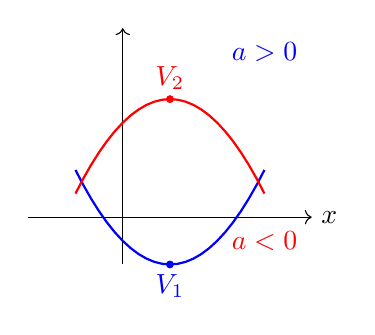
\begin{tikzpicture}[scale=0.6]
    \draw[->] (-2,0) -- (4,0) node[right]{$x$};
    \draw[->] (0,-1) -- (0,4);
    \draw[blue, thick] plot[domain=-1:3] (\x, {0.5*\x*\x - \x - 0.5});
    \draw[red, thick] plot[domain=-1:3] (\x, {-0.5*\x*\x + \x + 2});
    \filldraw[blue] (1,-1) circle (2pt) node[below]{$V_1$};
    \filldraw[red] (1,2.5) circle (2pt) node[above]{$V_2$};
    \node at (3,3.5) [blue] {$a>0$};
    \node at (3,-0.5) [red] {$a<0$};
\end{tikzpicture}
\end{center}

\section*{2. Função Exponencial}
$f(x) = a^x$ ou $f(x) = k \cdot a^{x} + c$

\subsection*{Características}
\begin{itemize}
    \item Crescente se $a>1$, decrescente se $0<a<1$
    \item Assíntota horizontal: $y = c$
    \item Intercepto y: $(0, k+c)$
    \item Não possui raízes reais em casos básicos
\end{itemize}

\begin{center}
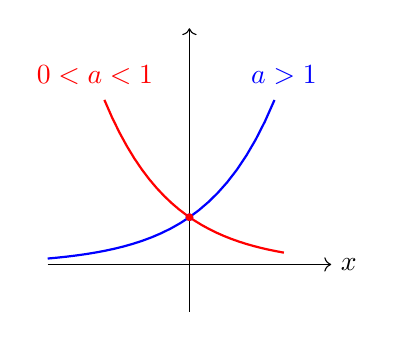
\begin{tikzpicture}[scale=0.6]
    \draw[->] (-3,0) -- (3,0) node[right]{$x$};
    \draw[->] (0,-1) -- (0,5);
    \draw[blue, thick] plot[domain=-3:1.8] (\x, {2^\x});
    \draw[red, thick] plot[domain=-1.8:2] (\x, {(0.5)^\x});
    \node at (2,4) [blue] {$a>1$};
    \node at (-2,4) [red] {$0<a<1$};
    \filldraw[blue] (0,1) circle (2pt);
    \filldraw[red] (0,1) circle (2pt);
\end{tikzpicture}
\end{center}

\section*{3. Comparação das Funções}

\begin{center}
\begin{tabular}{|l|l|l|}
\hline
 & Quadrática & Exponencial \\
\hline
Forma & Parábola & Curva suave \\
Domínio & $\mathbb{R}$ & $\mathbb{R}$ \\
Imagem & Depende de $a$ & $(c, +\infty)$ ou $(-\infty, c)$ \\
Crescimento & Até vértice & Monótona \\
Raízes & 0, 1 ou 2 & 0 ou 1 \\
\hline
\end{tabular}
\end{center}

\section*{4. Análise Gráfica}

\subsection*{Gràfico 1: Quadrática Completa}
\begin{center}
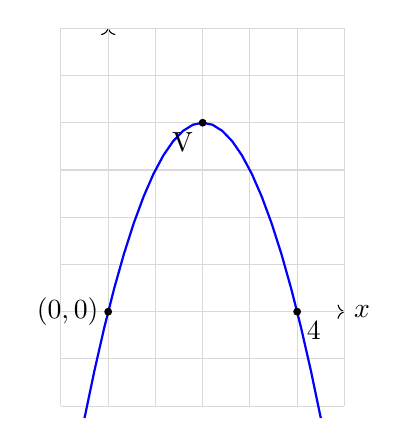
\begin{tikzpicture}[scale=0.6]
    \draw[->] (-1,0) -- (5,0) node[right]{$x$};
    \draw[->] (0,-2) -- (0,6);
    \draw[gray!30] (-1,-2) grid (5,6);
    \draw[blue, thick] plot[domain=-0.5:4.5] (\x, {-\x*\x + 4*\x});
    \filldraw (0,0) circle (2pt) node[left]{$(0,0)$};
    \filldraw (4,0) circle (2pt) node[below right]{4};
    \filldraw (2,4) circle (2pt) node[below left]{V};
\end{tikzpicture}

\textbf{Questões:}
\begin{enumerate}[label=\alph*)]
    \item Qual a concavidade?
    \item Quais as raízes?
    \item Qual o vértice?
\end{enumerate}
\end{center}

\subsection*{Gràfico 2: Exponencial Transformada}
\begin{center}
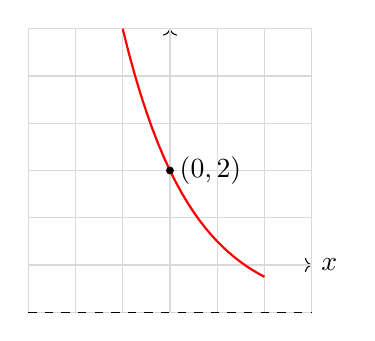
\begin{tikzpicture}[scale=0.6]
    \draw[->] (-3,0) -- (3,0) node[right]{$x$};
    \draw[->] (0,-1) -- (0,5);
    \draw[gray!30] (-3,-1) grid (3,5);
    \draw[red, thick] plot[domain=-1:2] (\x, {3*(0.5)^\x -1});
    \draw[dashed] (-3,-1) -- (3,-1);
    \filldraw (0,2) circle (2pt) node[right]{$(0,2)$};
\end{tikzpicture}

\textbf{Questões:}
\begin{enumerate}[label=\alph*)]
    \item A função é crescente ou decrescente?
    \item Qual $f(2)$ aproximado?
\end{enumerate}
\end{center}

\section*{5. Exercícios de Construção}

\subsection*{1. Esboce os gráficos de:}
\begin{enumerate}[label=\alph*)]
    \item $f(x) = x^2 - 4$
    \item $g(x) = 2^x$
    \item $h(x) = -x^2 + 2x + 3$
\end{enumerate}

\subsection*{2. Problemas Aplicados}
\begin{enumerate}
    \item O lucro de uma empresa é modelado por $L(t) = 50(1.2)^t - 50$, onde $t$ é o tempo em meses. Esboce o gráfico e determine:
    \begin{itemize}
        \item O lucro inicial ($t=0$)
        \item Quando o lucro atingirá 100?
    \end{itemize}
    
    \item Um projétil segue a trajetória $h(x) = -x^2 + 10x$, onde $h$ é a altura e $x$ a distância horizontal. Determine:
    \begin{itemize}
        \item A altura máxima
        \item O alcance (quando $h = 0$)
    \end{itemize}
\end{enumerate}

\section*{6. Análise de Funções Quadráticas e Exponenciais (Gráficos)}

\begin{center}
\textbf{Gráfico 1: Função Quadrática}
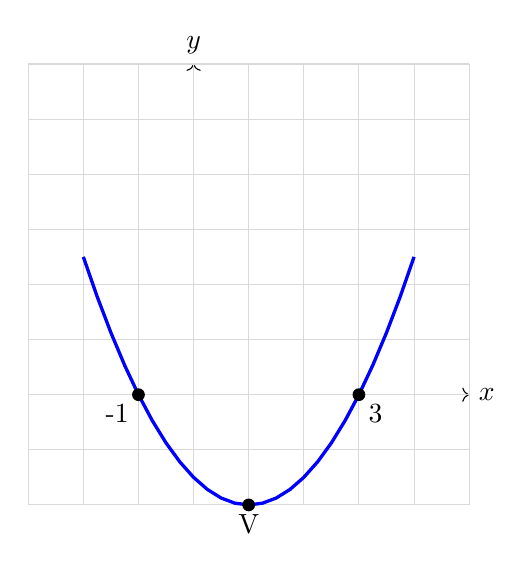
\begin{tikzpicture}[scale=0.7]
    \draw[->] (-3,0) -- (5,0) node[right]{$x$};
    \draw[->] (0,-2) -- (0,6) node[above]{$y$};
    \draw[gray!30] (-3,-2) grid (5,6);
    \draw[blue, very thick] plot[domain=-2:4] (\x, {0.5*\x*\x - \x - 1.5});
    \filldraw (3,0) circle (3pt) node[below right]{3};
    \filldraw (-1,0) circle (3pt) node[below left]{-1};
    \filldraw (1,-2) circle (3pt) node[below]{V};
\end{tikzpicture}

\vspace{0.3cm}
\textbf{Perguntas:}
\begin{enumerate}[label=\alph*)]
    \item Quais são as raízes da função?
    \item Quais as coordenadas do vértice V?
    \item Qual o valor de $y$ quando $x=2$?
    \item Para quais valores de $x$ a função é decrescente?
\end{enumerate}
\end{center}

\begin{center}
\textbf{Gráfico 2: Função Exponencial Crescente}
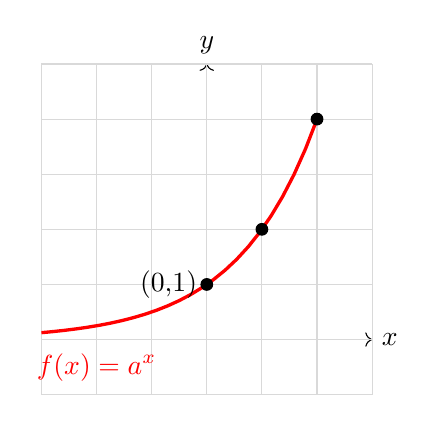
\begin{tikzpicture}[scale=0.7]
    \draw[->] (-3,0) -- (3,0) node[right]{$x$};
    \draw[->] (0,-1) -- (0,5) node[above]{$y$};
    \draw[gray!30] (-3,-1) grid (3,5);
    \draw[red, very thick] plot[domain=-3:2] (\x, {2^\x});
    \filldraw (0,1) circle (3pt) node[left]{(0,1)};
    \filldraw (1,2) circle (3pt);
    \filldraw (2,4) circle (3pt);
    \node at (-2,-0.5) [red]{$f(x)=a^x$};
\end{tikzpicture}

\vspace{0.3cm}
\textbf{Perguntas:}
\begin{enumerate}[label=\alph*)]
    \item Qual o valor de $f(0)$?
    \item A função é crescente ou decrescente?
    \item Qual o valor aproximado de $f(-1)$?
\end{enumerate}
\end{center}

\section*{7. Cálculo das Raízes da Equação do 2º Grau}

\subsection*{Fórmula Resolutiva (Bhaskara)}
Para a equação $ax^2 + bx + c = 0$, com $a \neq 0$, as raízes são dadas por:
\[
x = \frac{-b \pm \sqrt{\Delta}}{2a}
\]
onde o discriminante $\Delta = b^2 - 4ac$ determina a natureza das raízes:

\begin{itemize}
    \item $\Delta > 0$: Duas raízes reais distintas
    \item $\Delta = 0$: Uma raiz real dupla
    \item $\Delta < 0$: Não existem raízes reais
\end{itemize}

\subsection*{Exercícios Práticos}

\begin{enumerate}
    \item Calcule as raízes das equações:
    \begin{multicols}{2}
    \begin{enumerate}[label=\alph*)]
        \item $x^2 - 9 = 0$
        \item $2x^2 - 8x = 0$
        \item $x^2 + 4x + 4 = 0$
        \item $3x^2 - 7x + 2 = 0$
        \item $-x^2 + 6x - 9 = 0$
        \item $x^2 + 2x + 5 = 0$
    \end{enumerate}
    \end{multicols}
    
    \item Para cada caso, determine o valor de $k$ para que:
    \begin{enumerate}[label=\alph*)]
        \item $x^2 - kx + 9 = 0$ tenha raiz dupla
        \item $2x^2 + 3x + k = 0$ tenha duas raízes reais distintas
        \item $kx^2 + 4x + 1 = 0$ não tenha raízes reais
    \end{enumerate}
    
    \item Problema aplicado: Um jardim retangular tem área de 54 m². Se o comprimento é 3 m maior que a largura, quais são suas dimensões?
\end{enumerate}

\end{multicols}

\end{document}
